\chapter{Valid Outcomes of Positive Support Size One, Two, and Three}

\section{Invertibility Criterion}

In this section, we study the supports of valid outcomes; knowing that some supports cannot be the supports of valid outcomes will help us to prove Theorem \ref{thm:outcome-degree-support-size}. For instance, configurations that have support in the entries below marked with an \texttt{*} cannot be valid outcomes as we will see.
\begin{verbatim}
    ·  
    ·  · 
    *  ·  · 
    ·  ·  ·  · 
    ·  ·  ·  ·  · 
    ·  ·  ·  ·  *  · 
    *  ·  *  ·  ·  *  *
\end{verbatim}
The most important tool in the study of supports of valid outcomes is the \emph{Invertibility Criterion}, which we will present in this chapter. It was first investigated in \cite{bik2022classifying}. 

First, let us introduce a new basis for the space of Pascal forms.

\begin{definition}
    Let \( k = 0, \dots, d \) and \( \mathbf e_k \in \mathbb{R}^{d+1} \) be the \( k \)-th unit vector. We define \( \mathrm{diag}(k) \) to be the unique Pascal form \( \sum c_{i,j}x_{i,j} \) such that \( c_{k,d-k} = \mathbf e_k \).
\end{definition}

\begin{example}
    Fix the degree \( d = 7 \). We visualize \( \mathrm{diag}(3) \) by
    \begin{verbatim}
        .
        .   .
        .   .   .
        1   1   1   1
        4   3   2   1   .
       10   6   3   1   .   .
       20  10   4   1   .   .   . 
       35  15   5   1   .   .   .   .
    \end{verbatim}
\end{example}

\begin{proposition}\label{prop:diagonal-basis-324324324231}
    For all integers \( k = 0, \dots, d \) we have \( \mathrm{diag}(k)  = \sum_{(i,j) \in V_d}\binom{d - i - j}{k-i} x_{i,j} \).
\end{proposition}

\begin{proof}
    Note that for all \( (i,j) \in V_d \) with \( i+j = d \) we have \( \binom{d - i - j}{k-i} = 1 \) if and only if \( k= i \), and in all other cases \( k \neq i \) the binomial coefficient is zero. Thus, it remains to show that \( \sum_{(i,j) \in V_d}\binom{d - i - j}{k-i} x_{i,j} \) is a Pascal form. We have \(  \binom{d-i-j}{k-i} = \binom{d-i-1-j}{k-i-1} + \binom{d-i-j-1}{k-i} \)
    for all \( (i,j) \in V_{d-1} \) because \( \binom{a+1}{b+1} = \binom{a}{b+1} + \binom{a}{b}\).
\end{proof}

\begin{proposition}
    Let \( p \) be a Pascal form on \( \mathbb Z^{V_d} \). There exist unique coefficients \( \mu_0, \dots, \mu_d \in \mathbb{Z} \) such that 
    \( p = \mu_0 \mathrm{diag}(0) + \dots + \mu_d \mathrm{diag}(d) \).
\end{proposition}

\begin{proof}
    Let \( p = \sum c_{i,j}x_{i,j} \). Choose \( \mu_k = c_{k,d-k} \) for \( k=0, \dots, d \). Since \( p \) is a Pascal form, the coefficients \( c_{i,j} \) satisfy the Pascal recurrence relation. Thus, the coefficients \( \mu_k \) are uniquely determined.
\end{proof}

Given \( S \subset V_d \), the Invertibility Criterion uses the diagonal basis \( (\mathrm{diag}(0), \dots, \mathrm{diag}(d)) \) to determine whether a nonzero outcome with support in \( S \) exists.

\begin{definition}\label{def:pairing-matrix}
    Let \( d \in \mathbb{N} \), \( E \subset \left\{ 0, \dots, d \right\} \), and \( S \subset V_d \) be non-empty sets such that \( \lvert E \rvert = \lvert S \rvert \) holds. The \emph{pairing matrix} of \( (E,S) \) is defined as \( A^{(d)}_{E,S} \coloneqq \begin{bmatrix} \binom{d-i-j}{k-i} \end{bmatrix}_{k \in E, (i,j) \in S} \).
\end{definition}

\begin{example}
    Let \( d = 2 \), \( S = \left\{ (1,1), (0,0) \right\} \), and \( E = \left\{ 0,1 \right\} \). The pairing matrix reads \(  A^{(d)}_{E,S}  = \begin{bmatrix}
        \binom{2-1-1}{0-1} & \binom{2-0-0}{0-2} \\
        \binom{2-1-1}{1-1}  & \binom{2-0-0}{1-2}
    \end{bmatrix} = \begin{bmatrix}
        0 & 0 \\
        1 & 0
    \end{bmatrix} \). Now, assume that \( \mathbf{w} \) is an outcome with support in \( S \). Since it is an outcome, we have \( \mathrm{diag}(k)(\mathbf{w}) = 0 \) for all \( k = 0, 1,2,3 \). Thus, we have \(  A^{(d)}_{E,S} \mathbf w = \mathbf 0 \).
\end{example}

We make the following observation: if the pairing matrix \( A^{(d)}_{E,S} \) is invertible (it is not for the example above), then \( A^{(d)}_{E,S} \mathbf w = \mathbf 0 \) if and only if \( \mathbf w = \mathbf 0 \); so an invertible pairing matrix means that the initial configuration \( \mathbf{0} \) is the \emph{only} outcome with support in \( S \). This is the Invertibility Criterion. For the example above, this criterion is inconclusive since the pairing matrix is not invertible.

\begin{proposition}[Invertibility Criterion]
    Let \( \mathbf{w} \) be an outcome with \( \mathrm{supp}(\mathbf w) \subset S \).
    If \( A^{(d)}_{E,S} \) is invertible, then \( \mathbf{w} = \mathbf 0 \).
\end{proposition}

\begin{proof}[Proof by Contraposition]
    Let \( \mathbf{w} \neq \mathbf 0 \). Its support is non-empty. Then, \( \mathbf w' \coloneqq (w_{i,j})_{(i,j) \in S} \neq \mathbf 0 \). So, \( A^{(d)}_{E,S} \cdot \mathbf w' = \mathbf 0 \). The kernel of the pairing matrix is non-trivial. Hence, the pairing matrix \( A^{(d)}_{E,S} \) is not invertible.
\end{proof}

Given a non-zero configuration \( \mathbf{w} \), we try to construct sets \( S \supset \mathrm{supp}(\mathbf w) \) and \( E \) such that the pairing matrix \( A_{E,S}^{(d)} \) is invertible. If we succeed, then \( \mathbf{w} \) is \emph{not} an outcome since the initial configuration is the only valid outcome with support in \( S \). 


The Invertibility Criterion inspires the following algorithm for determining if a set of indices \( S \subset V_d \) can actually be the support of some nonzero outcome in \( \mathbb{Z}^{V_d} \). It is later used in the proof of Theorem \ref{thm:main-result-32432432432nkdnjkfd} and Proposition \ref{prop:uiwuwinca}.

\begin{algorithm}[H]
\caption{Only Zero Outcome}\label{alg:hyperfield_criterion:is_zero}
    \begin{algorithmic}[1]
    \Require Support set $S \subset {V_d}$
    \Ensure \texttt{True} only if \( \mathbf{0} \) is the only outcome \( \mathbf{w} \) with \( \mathrm{supp}(\mathbf{w}) \subset S \), \texttt{False} if inconclusive

    \State $\texttt{E} \gets \{0, \dots, |{S}| - 1\}$
    \State $\texttt{P} \gets \texttt{build\_pairing\_matrix}(d, \texttt{E}, S)$    
    \State \Return $\texttt{rank}(\texttt{P}) = |S|$
    \end{algorithmic}  
\end{algorithm}

The function \texttt{build\_pairing\_matrix} constructs the pairing matrix \( A^{(d)}_{E,S} \) as defined in Definition \ref{def:pairing-matrix}. If this algorithm is inconclusive, we try another set \( E \subset \left\{ 0, \dots, d \right\} \). This leads to the following generalization:

\begin{algorithm}[H]
\caption{Only Zero Outcome (Generalized)}\label{alg:hyperfield_criterion:is_zero_general}
    \begin{algorithmic}[1]
    \Require Support set $S \subset {V_d}$, set \( E \subset \left\{ 0, \dots, d \right\} \) with size \( \lvert S \vert \)
    \Ensure \texttt{True} only if \( \mathbf{0} \) is the only outcome \( \mathbf{w} \) with \( \mathrm{supp}(\mathbf{w}) \subset S \), \texttt{False} if inconclusive

    \State $\texttt{P} \gets \texttt{build\_pairing\_matrix}(d, \texttt{E}, S)$    
    \State \Return $\texttt{rank}(\texttt{P}) = |S|$
    \end{algorithmic}  
\end{algorithm}
The first algorithm is clearly a special case of the second algorithm with \( E =  \{0, \dots, |{S}| - 1\}\).

\section{Divide and Conquer}\label{sec:divide-and-conquer}

The Invertibility Criterion is a powerful tool to determine whether a configuration is an outcome. Unfortunately, it is not always easy to find suitable sets \( S \) and \( E \). We will now introduce a method to construct such sets.

\subsection*{Divide}\label{subsec:divide}

Instead of finding one set \( S \) with \( \mathrm{supp}(\mathbf w) \subset S \), we divide \( S \) into smaller sets \( S_1, \dots, S_l \). These smaller sets \( S_1, \dots, S_k \) are implicitly defined by integers \( \lambda_1, \dots, \lambda_l \in \mathbb{N} \). We choose \( l \in \mathbb{N} \) and integers \( \lambda_1, \dots, \lambda_l \in \mathbb{N} \) such that for all \( i=1, \dots, d \) we have 
\begin{itemize}
    \item \( \lvert S_i \rvert \in \left\{ 0, \lambda_i \right\} \), 
    \item \( S_i \coloneqq \left\{ (i,j) \in \mathrm{supp}(\mathbf w) : i = c_{k-1}, \dots, c_k - 1 \right\} \),
    \item  \( c_i \coloneqq \lambda_1 + \dots + \lambda_i\), and
    \item \(  \lambda_1 + \dots + \lambda_l = d+1 \).
\end{itemize}
Moreover, for all \( i=1, \dots, l \) we define the sets \( E_i \coloneqq \begin{cases}
    \left\{ c_{i-1}, \dots, c_i - 1 \right\} & \text{if } \lvert S_i \rvert = \lambda_i, \\
    \emptyset & \text{if } \lvert S_i \rvert = 0
\end{cases} \).

\begin{remark}\label{rem:ksldmfiewonowiniew}
This decomposition works if \( \lvert \left\{ (i,j) \in \mathrm{supp}(\mathbf{w}) : i \geq d-k \right\} \rvert \leq k+1 \) for all \( k = 0, \dots, d \). This is because we can always choose \( \lambda_1  \) minimal such that \( \lvert S_1 \rvert \in \left\{ 0, \lambda_1 \right\} \). We repeat this process until \( c_l = d+1 \). 
\end{remark}

\begin{remark}
    We see that \( \lvert E_i \rvert = \lvert S_i \rvert \) for all \( i = 1, \dots, l \). 
\end{remark}

\begin{example}\label{ex:decomposition-nsjkfnje}
    Fix the degree \( d=6 \). Assume we have some configuration \( \mathbf w \in \mathbb{Z}^{V_6} \) with support in the positions marked with an \texttt{*} below. The first column contains two non-zero entries. So, we set \( \lambda_1 = 2 \). Then, we conclude that \( \lambda_2 = \lambda_3 = \lambda_4 = \lambda_5 = \lambda_6 = 1\).
    \begin{verbatim}
        · 
        · · 
        * · · 
        · · · · 
        · · · · · 
        · · · · * · 
        * · * · · * *
    \end{verbatim}
\end{example}

We present the following algorithm that implements this division rule.


\begin{algorithm}[H]
\caption{Divide}
\label{alg:divide}
\begin{algorithmic}[1]
\Require \( S \subset V_d \)
\Ensure \( L \in \mathbb{Z}^{k} \) where \( L_i = \lvert S_i \rvert \) if a division \( (\lambda, (E_i)_{i=1}^k, (S_i)_{i=1}^k) \) is found; \texttt{None} otherwise

\State $R \gets [0, \dots, d]$, $L \gets \texttt{list()}$, and $\texttt{col\_start} \gets 0$

\For{$\texttt{col\_end} \in \{0, \dots, |R|-1\}$}
    \State $\texttt{num\_cols} \gets \texttt{col\_end} - \texttt{col\_start} + 1$
    \State $\texttt{points\_in\_col} \gets \{(x,y) \in S \mid x \in \{R[\texttt{col\_start}], \dots,  R[\texttt{col\_end}] \} \}$
    \State $\texttt{num\_points} \gets |\texttt{points\_in\_col}|$

    \If{$(\texttt{num\_points} = 0) \lor (\texttt{num\_cols} = \texttt{num\_points})$}
        \State $L.\texttt{append}(\texttt{num\_points})$
        \State $\texttt{col\_start} \gets \texttt{col\_end} + 1$
    \EndIf
\EndFor

\If{$\sum_{i=1}^k L_i \neq \lvert S \rvert$}
    \State \Return \texttt{None}
\EndIf

\State \Return $L$
\end{algorithmic}
\end{algorithm}

\begin{proof}[Proof of Correctness]
    To construct \( \lambda  \) from \( S \), we set \( \lambda_i = L_i \) if \( L_i > 0 \), otherwise \( \lambda_i = 1 \).
    Line four guarantees that \( S_i \coloneqq \left\{ (i,j) \in S : i = c_{k-1}, \dots, c_k - 1 \right\} \). Line six states that \( \lvert S_i \rvert \) is appended to \( L \) if and only if either \( S_i = \emptyset \) or \( \lvert S_i \rvert = \lambda_i \). Line eleven ensures that \(  \lambda_1 + \dots + \lambda_l = d+1  \).
\end{proof}




\subsection*{Conquer}

It remains to show how to conquer all the sets \( S_1, \dots, S_l \) and \( E_1, \dots, E_l \).

\begin{proposition}
    We have \( A_{E,S}^{(d)} = 
    \begin{bmatrix}
        A_{E_1,S_1}^{(d)} & 0 & \dots & 0 \\
        A_{E_2,S_1}^{(d)} & A_{E_2,S_2}^{(d)} & \dots & 0 \\
        \vdots & \vdots & \ddots & \vdots \\
        A_{E_l,S_1}^{(d)} & A_{E_l,S_2}^{(d)} & \dots & A_{E_l,S_l}^{(d)}
    \end{bmatrix} \).
\end{proposition}

\begin{proof}
    First, note that 
    \begin{align*}
        A_{E,S}^{(d)} = 
        \begin{bmatrix}
            A_{E_1,S_1}^{(d)} & A_{E_1,S_2}^{(d)} & \dots & A_{E_1,S_l}^{(d)} \\
            A_{E_2,S_1}^{(d)} & A_{E_2,S_2}^{(d)} & \dots & A_{E_2,S_l}^{(d)} \\
            \vdots & \vdots & \ddots & \vdots \\
            A_{E_l,S_1}^{(d)} & A_{E_l,S_2}^{(d)} & \dots & A_{E_l,S_l}^{(d)}
        \end{bmatrix}.
    \end{align*}
    Let \( x,y = 1, \dots , l \) such that \( x < y \). Let \( k \in E_x \) and \( (i,j) \in S_y \).
    Then, \( k \leq c_x - 1 < c_x \leq c_{y - 1} \leq i \); so \( k - i < 0 \). Thus, \( \binom{d-i-j}{k-i} = 0 \) holds. This implies that the upper off-diagonal blocks are zero.
\end{proof}

\begin{corollary}
    The matrix \( A^{(d)}_{E,S} \) is invertible if and only if \( A^{(d)}_{E_1,S_1}, \dots,  A^{(d)}_{E_l,S_l} \) are invertible.
\end{corollary}

\begin{corollary}[Invertibility Criterion, Divide and Conquer]\label{cor:invertibility-criterion-nooos}
    Let \( \mathbf{w} \) be an outcome with \( \mathrm{supp}(\mathbf w) \subset S \).
    If \( A^{(d)}_{E_1,S_1}, \dots,  A^{(d)}_{E_l,S_l} \) are invertible, then \( \mathbf{w} = \mathbf 0 \).
\end{corollary}

\begin{example}
    We continue Example \ref{ex:decomposition-nsjkfnje}. Choose \( \lambda = (2,1,1,1,1,1) \). Then, we obtain 
    \begin{gather*}
        S_1 = \left\{ (0,0), (0,4) \right\}, S_2 = \left\{ (2,0) \right\}, S_3 = \emptyset, S_4 = \left\{ (4,1) \right\}, S_5 = \left\{ (5,0) \right\}, S_6 = \left\{ (6,0) \right\},\\
        E_1 = \left\{ 0, 1 \right\}, E_2 = \left\{ 2 \right\}, E_3 = \emptyset, E_4 = \left\{ 4 \right\}, E_5 = \left\{ 5 \right\}, E_6 = \left\{ 6 \right\}\\
        A^{(d)}_{E,S} = \begin{bmatrix}
            1 & 1 & 0 & 0 & 0 & 0 \\
            6 & 2 & 0 & 0 & 0 & 0 \\
            * & * & 1 & 0 & 0 & 0 \\
            * & * & * & 1 & 0 & 0 \\
            * & * & * & * & 1 & 0 \\
            * & * & * & * & * & 1
        \end{bmatrix}.
    \end{gather*}
    The symbol \( * \) stands for arbitrary entries. The pairing matrix is invertible, so no nonzero outcome with support in \( S = \left\{ (0,0), (0,4), (2,0), (4,1), (5,0), (6,0) \right\} \) exists.
\end{example}

\section{Symmetry}\label{sec:symmetry}

With the Invertibility Criterion we exclude certain supports from being supports of valid outcomes. We now show that supports of valid outcomes are invariant under certain symmetries.

\begin{proposition}\label{prop:symmetry}
    Let \( \mathbf{w} = (w_{i,j})_{(i,j) \in V_d} \) be a configuration in \( \mathbb{Z}^{V_d} \). Then \( \mathbf{w} \) is an outcome if and only if  the configuration \(  \tilde{\mathbf{w}} \coloneqq (w_{j,i})_{(i,j) \in V_d} \) is an outcome.
\end{proposition}

\begin{proof}
    Let \(  k = 0, \dots, d \) and \(\mathbf{w} \) be a valid outcome.
    Observe that
    \begin{align*}
        \mathrm{diag}(k)  = \sum_{(i,j) \in V_d}\binom{d - i - j}{k-i} x_{i,j}
        = \sum_{(i,j) \in V_d}\binom{d - i - j}{d-i-j-(k-i)} x_{i,j}
        = \sum_{(i,j) \in V_d}\binom{d - i - j}{d-k-j} x_{i,j}.
    \end{align*}
    Then, \( \mathrm{diag}(k)(\mathbf{w}) = 0 \) holds. Thus, we have
    \begin{align*}
        \mathrm{diag}(k)(\tilde{\mathbf{w}}) = \sum_{(i,j) \in V_d}\binom{d - i - j}{k-j} w_{j,i}
        = \sum_{(i,j) \in V_d}\binom{d - i - j}{d-k-i} w_{j,i}
        &= \sum_{(i,j) \in V_d}\binom{d - i - j}{d-k-j} w_{i,j} \\
        &= \sum_{(i,j) \in V_d}\binom{d - i - j}{k-i} w_{i,j} \\
        &= \mathrm{diag}(k)(\mathbf w) = 0.
    \end{align*}
\end{proof}

\begin{example}
    We have established that the support on the left-hand side cannot correspond to a valid outcome. By symmetry, the support on the right-hand side also does not correspond to a valid outcome.
    \begin{verbatim}
·                      *
· ·                    * ·
* · ·                  · * · 
· · · ·                · · · · 
· · · · ·              * · · · · 
· · · · * ·            · · · · · ·
* · * · · * *          * · · · * · ·
    \end{verbatim}
\end{example}

Next, we introduce another kind of symmetry. Let \( \mathbf{w} = (w_{i,j}) \) be a configuration in \( \mathbb{Z}^{V_d} \). We define \( \mathbf w \mapsto \hat{\mathbf w} \coloneqq \left( (-1)^{d-j} w_{j, d - i -j} \right)_{(i,j) \in V_d} \).

\begin{proposition}\label{prop:symmetry-2}
    Let \( \mathbf{w} = (w_{i,j})_{(i,j) \in V_d} \) be a configuration in \( \mathbb{Z}^{V_d} \). Then \( \mathbf{w} \) is an outcome if and only if \( \hat{\mathbf w} \coloneqq \left( (-1)^{d-j} w_{j, d - i -j} \right)_{(i,j) \in V_d} \) is an outcome.
\end{proposition}

\begin{proof}
    Let \( k = 0, \dots, d \). Then, we have \( \mathrm{col}(k)(\hat{\mathbf w}) = (-1)^k \sum_{(i,j) \in V_d}(-1)^j \binom{i}{k-j}(-1)^{d-j}w_{j, d-i-j} 
    = (-1)^{d-k} \sum_{(i,j) \in V_d}\binom{d-i-j}{k-i}w_{i, j} 
    = (-1)^{d-k} \mathrm{diag}(k)(\mathbf w) = 0 \).
\end{proof}

The symmetry just introduced is interpreted in the following way: we define a group action of the symmetry group \( S_3 \) on \( \mathbb{Z}^{V_d} \) by \( (12) \cdot \mathbf w = \tilde{\mathbf w}  \) and \( (123) \cdot \mathbf w = \hat{\mathbf w} \).
The group actions \( (12) \), \( (13) \) and \( (23) \) can then be depicted in Figure \ref{fig:group-action-s3}.

\begin{figure}[H]
    \centering
    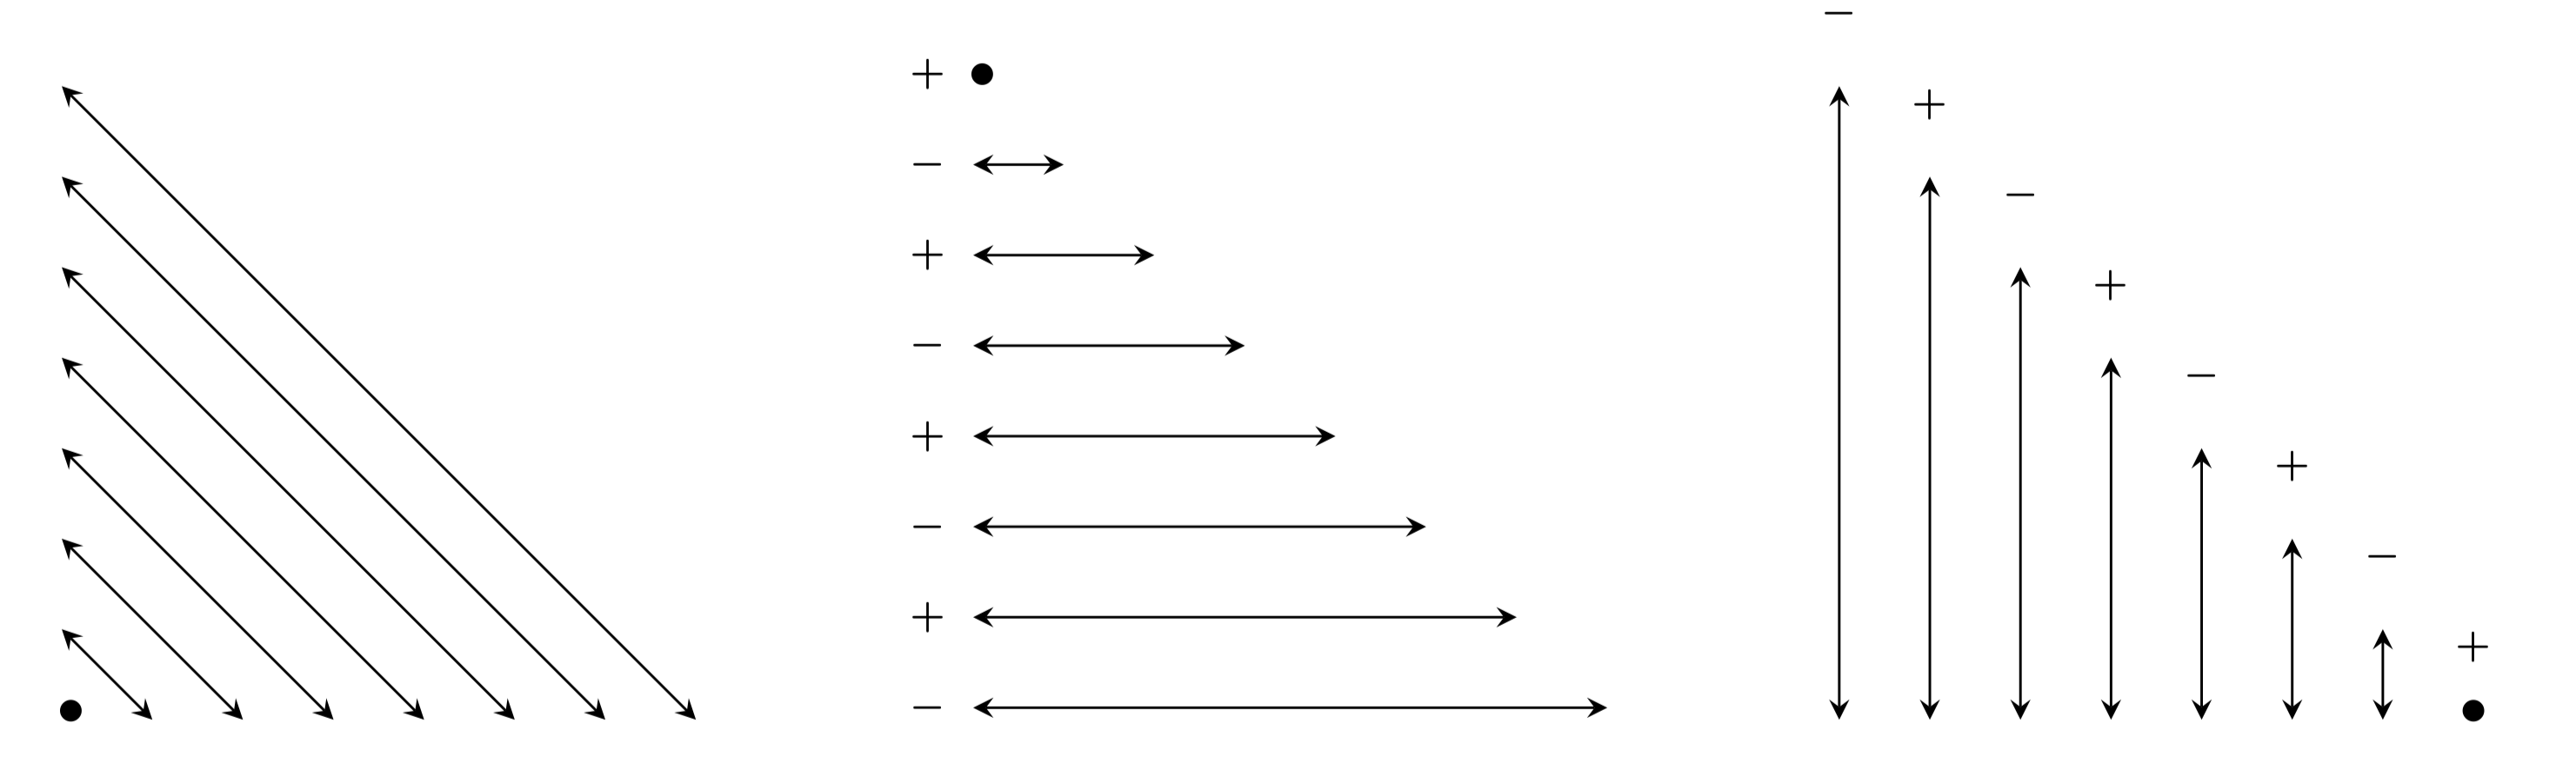
\includegraphics[width=0.8\textwidth]{assets/group-action-s3.png}
    \caption{The left most illustration shows mirroring the configuration with respect to the main diagonal. The middle illustration shows switching the order on the same row while also alternating the signs of the row. The right most illustration shows switching the order on the same column while also alternating the signs of the column.}
    \label{fig:group-action-s3}
\end{figure}

\section{Impossible Supports}\label{sec:impossible-supports}

We show that certain supports cannot be the supports of valid outcomes. 

\begin{proposition}\label{prop:impossible-support-23233243243423}
    Let \( d \in \mathbb{N} \), and \( i=0, \dots, d \). If \( S = \left\{ (0,i) \right\} \) and \( E = \left\{ 0 \right\} \), then \( A^{(d)}_{E,S} \) is invertible.
\end{proposition}

\begin{proof}
    We have \( A^{(d)}_{E,S} = \begin{bmatrix}
        1
    \end{bmatrix} \), which is invertible.
\end{proof}

\begin{proposition}\label{prop:impossible-support-232423}
    Let \( d \in \mathbb{N} \). Assume \( i,j=0, \dots, d \) with \( i < j \). If \( S = \left\{ (0,i), (0,j) \right\} \) and \( E = \left\{ 0,1 \right\} \), then \( A^{(d)}_{E,S} \) is invertible.
\end{proposition}

\begin{proof}
    We have \( A^{(d)}_{E,S} = \begin{bmatrix}
        1 & 1 \\ d-i & d-j
    \end{bmatrix} \), which is invertible.
\end{proof}

\begin{proposition}\label{prop:impossible-support-2}
    Let \( d \in \mathbb{N} \). Assume \( i,j,k=0, \dots, d \) with \( i < j < k \). If \( S = \left\{ (0,i), (0,j), (0,k) \right\} \) and \( E = \left\{ 0,1,2 \right\} \), then \( A^{(d)}_{E,S} \) is invertible.
\end{proposition}

\begin{proof}
    We have  \( A^{(d)}_{E,S} = \begin{bmatrix}
        \binom{d-i}{0} & \binom{d-j}{0} & \binom{d-k}{0} \\
        \binom{d-i}{1} & \binom{d-j}{1} & \binom{d-k}{1} \\
        \binom{d-i}{2} & \binom{d-j}{2} & \binom{d-k}{2}
    \end{bmatrix} = \begin{bmatrix}
        1 & 1 & 1 \\
        d-i & d-j & d-k \\
        \frac{(d-i)(d-i-1)}{2} & \frac{(d-j)(d-j-1)}{2} & \frac{(d-k)(d-k-1)}{2}
    \end{bmatrix} \).
    We set \( x = d-i, y = d-j \), and \( z = d-k \).
    Then, we see \( \begin{bmatrix}
        1 & 0 & 0 \\
        0 & 1 & 0 \\
        0 & 1 & 2
    \end{bmatrix}A^{(d)}_{E,S} = \begin{bmatrix}
        1 & 1 & 1 \\
        x & y & z \\
        x^2 & y^2 & z^2
    \end{bmatrix} \).
    The matrix on the right-hand side is invertible because it is a Vandermonde matrix. Thus, \( A^{(d)}_{E,S} \) is invertible.
\end{proof}

\begin{proposition}\label{prop:impossible-support-2324223423123123}
    Let \( d \in \mathbb{N} \), \( i,j=0, \dots, d \) with \( i < j \), and \( k=0, \dots, d-1 \). If we have \( S = \left\{ (0,i), (0,j), (1,k) \right\} \), \( E = \left\{ 0,1,2 \right\} \), and \( i+j \neq 2k + 1 \), then \( A^{(d)}_{E,S} \) is invertible.
\end{proposition}

\begin{proof}
    We have 
    \begin{align*}
        A^{(d)}_{E,S} = \begin{bmatrix}
            \binom{d-i}{0} & \binom{d-j}{0} & \binom{d-k-1}{-1} \\
            \binom{d-i}{1} & \binom{d-j}{1} & \binom{d-k-1}{0} \\
            \binom{d-i}{2} & \binom{d-j}{2} & \binom{d-k-1}{1}
        \end{bmatrix} = \begin{bmatrix}
            1 & 1 & 0 \\
            d-i & d-j & d-k-1 \\
            \frac{(d-i)(d-i-1)}{2} & \frac{(d-j)(d-j-1)}{2} & \frac{(d-k-1)(d-k-2)}{2}
        \end{bmatrix}.
    \end{align*}
    We substitute \( x = d-i, y = d-j \), and \( z = d-k-1 \).
    Then, we see 
    \begin{align*}
        \begin{bmatrix}
            1 & 0 & 0 \\
            0 & 1 & 0 \\
            0 & 1 & 2
        \end{bmatrix}
        A^{(d)}_{E,S} \begin{bmatrix}
            1 & 1 & 0 \\
            0 & -1 & 0 \\
            0 & 0 & 1
        \end{bmatrix}
        \begin{bmatrix}
            1 & 0 & 0 \\
            0 & \frac{1}{x-y} & 0 \\
            0 & 0 & 1
        \end{bmatrix} = 
        \begin{bmatrix}
            1 & 0 & 0 \\
            x & 1 & 1 \\
            x^2 & x+y & 2z+1
        \end{bmatrix}.
    \end{align*}
    We see that the determinant is nonzero because \( x + y \neq 2z + 1 \) by \( i+j \neq 2k+1 \).
\end{proof}

\begin{remark}\label{rem:generality-jfknwejn}
    We may assume \(  S \subset \left\{ (i,j) \in V_d \mid i < \lvert S \rvert \right\} \) and \( E = \left\{ 0,1, \dots, \lvert S \rvert - 1 \right\} \)
because \( A^{(d)}_{E,S} = A^{(d-\rho)}_{E - \rho, S - \rho} \) holds for \( \rho \coloneqq \min \left\{ E \cup \left\{ i \mid (i,j) \in S \right\} \right\} \) and \( E - \rho \coloneqq \left\{ (i - \rho, j) \mid (i,j) \in E \right\} \). This allows us to apply the previous propositions to more general \( S \) and \( E \).
\end{remark}

\begin{example}
    Assume we have a configuration with support \( S = \left\{ (0,i), (0,j), (0,k) \right\} \) for \( 0 \leq i < j< k \leq d \). By Proposition \ref{prop:impossible-support-2}, we know that no valid outcome has this support. Now, let us consider a configuration \( \mathbf{w} \) with support \( \mathrm{supp}(\mathbf{w}) \subset S \) such that \( S \) can be decomposed into \( S_1, \dots, S_l \) as described before. Let \( \ell = 1, \dots, l \). If \( S_\ell = \left\{ (x,i), (x,j), (x,k) \right\} \) for \( 0 \leq i < j< k \leq d \) and \( x \in \mathbb{N} \), then \( \mathbf{w} = \mathbf 0 \) by Proposition \ref{prop:impossible-support-2} and Remark \ref{rem:generality-jfknwejn}. Hence, the configuration below is not an outcome because for \( \lambda = (3,3,1,1) \) we have \( S_2 = \left\{ (3,0), (3,1), (3,3) \right\} \).
    \begin{verbatim}
                            *
                            .  .
                            .  .  *  
                            .  .  .  .  
                            .  .  .  *  .  
                            .  .  .  .  .  .  
                            .  .  .  *  .  .  .  
                            *  .  .  *  .  .  .  .  
    \end{verbatim}
\end{example}

\section{Proof}

We have all the tools to prove our north star (Theorem \ref{thm:outcome-degree-support-size}) for the case of positive support size three or less.

\begin{theorem}\label{thm:outcome-degree-support-size-232323}
    No valid outcomes of positive support size one exists.
\end{theorem}


\begin{proof}[Proof of Theorem \ref{thm:outcome-degree-support-size-232323}]
    Let \( \mathbf{w} \in \mathbb{Z}^{V_d} \) be a valid outcome. Since it is valid, we either have an empty negative support or a negative support that only contains \( (0,0) \). If the negative support is empty, then \( \mathbf{w} = \mathbf 0 \) by Proposition \ref{prop:outcome-zero}. Hence, we assume \( w_{0,0} < 0 \).

    Now, consider the Pascal form \( \mathrm{diag}(0) = \sum c_{i,j} x_{i,j} \). We have \( c_{0, 0} = c_{0, 1} = \dots = c_{0, d} = 1 \) and \( c_{i,j} = 0 \) for everything else. Similarly, we have for the Pascal form \( \mathrm{diag}(d) = \sum c'_{i,j} x_{i,j} \) that \( c'_{\cdot, 0} = \mathbf 1 \) and \( c'_{i,j} = 0 \) for everything else. Since outcomes are roots of Pascal forms, we have \( \mathrm{diag}(0)(\mathbf w) = \mathrm{diag}(d)(\mathbf w) = 0 \).
    Since \( w_{0,0} < 0 \) we must have \( w_{0,j} > 0 \) and \( w_{i, 0} > 0 \) for some \( i,j > 0 \). Hence, \( \mathbf{w} \) has positive support size at least two.
\end{proof}

\begin{theorem}\label{thm:outcome-degree-support-size-232323343}
    For valid outcomes \( \mathbf w \in \mathbb{Z}^{V_d} \) with \( |\mathrm{supp}^+(\mathbf w)| = 2 \) we have \( \mathrm{deg}(\mathbf w) = 1 \).
\end{theorem}


\begin{proof}[Proof of Theorem \ref{thm:outcome-degree-support-size-232323343}]
    Let \( \mathbf{w} \in \mathbb{Z}^{V_d} \) be an outcome with positive support size two and degree \( d \).
    By the previous proof, we see that \( \mathrm{supp}^+({\mathbf{w}}) = \left\{  (0,j), (i,0) \right\} \). Without loss of generality, we assume \( i = d \). We want to show that \( j = d \). 
    
    Consider the Pascal form \( \mathrm{row}(d) = \sum c_{i,j} x_{i,j} \); it satisfies \( c_{i,j} \neq 0 \) if and only if \( i + j = d \). If \( d \) is odd, we have \( c_{d,0} = 1 \) and \( c_{0,d} = -1 \). Since \( \mathrm{row}(d)(\mathbf{w}) = 0 \), we have \( j = d \). If \( d \) is even, we have \( c_{d,0} = c_{0,d} = 1 \). Thus, \( \mathrm{row}(d)(\mathbf w) \neq 0 \) for all \( j = 0, \dots, d \). Hence, valid outcomes with positive support size two do not exist for even degrees.

    From now on, we assume \(         \mathrm{supp}^+({\mathbf{w}}) = \left\{  (0,d), (d,0) \right\}    \).
    For sake of contradiction, let \( d \geq 2 \). Then, we divide \( \mathrm{supp}({\mathbf{w}}) = \left\{  (0,0) , (0,d), (d,0) \right\} \)
    via \( \lambda = (2,1,\dots,1) \) to obtain \( S_1 = \left\{ (0,0), (0,d) \right\} \), \( S_k = \emptyset \), and \( S_l = \left\{ (d,0) \right\} \) for some \( l \in \mathbb{N} \) and all \( k \neq l, k \neq 1 \). By Proposition \ref{prop:impossible-support-232423}, the pairing matrix induced by \( S_1 \) and \( E_1 = \left\{ 0,1 \right\} \) is invertible. For \( S_l \) we apply Proposition \ref{prop:impossible-support-23233243243423} to get that the induced pairing matrix is invertible. By Corollary \ref{cor:invertibility-criterion-nooos}, the outcome \( \mathbf{w} \) is zero, which has an empty positive support. This is a contradiction to the assumption that the positive support size is two. Hence, the degree \( d \) equals one.
\end{proof}

\begin{example}
    The previous theorem shows that the only valid outcomes with positive support size two are multiples of
    \begin{verbatim}
         1
        -1  1
    \end{verbatim}
\end{example}

We now turn our attention to valid outcomes with positive support size three.

\begin{theorem}\label{thm:sfnjksnfjkwenjfk}
    For valid outcomes \( \mathbf w \in \mathbb{Z}^{V_d}  \) with \( |\mathrm{supp}^+(\mathbf w)| = 3 \) we have \( \mathrm{deg}(\mathbf w) \leq 3 \).
\end{theorem}

The following proposition gives us the possible supports of valid outcomes with positive support size three.

\begin{proposition}\label{lemma:wmrkwjnr3w}
    Let \( \mathbf{w} \in \mathbb{Z}^{V_d} \) be a valid integral outcome of degree \( d \in \mathbb{N} \). If the positive support size of \( \mathbf{w} \) is three, then one of the following holds:
    \begin{enumerate}
        \item We have \( \mathrm{supp}(\mathbf{w}) = \left\{ (0,0), (d,0), (0,d), (i,j) \right\} \) for some \( i,j > 0 \) with \( i+j < d \).
        \item We have \( \mathrm{supp}(\mathbf{w}) = \left\{ (0,0), (d,0), (0,d), (i,d-i) \right\} \) for some \( i = 1, \dots, d-1 \).
        \item We have \( \mathrm{supp}(\mathbf{w}) = \left\{ (0,0), (d,0), (0,d), (i,0) \right\} \) for some \( i = 1, \dots, d-1 \).
        \item We have \( \mathrm{supp}(\mathbf{w}) = \left\{ (0,0), (d,0), (0,d), (0,i) \right\} \) for some \( i = 1, \dots, d-1 \).
        \item We have \( \mathrm{supp}(\mathbf{w}) = \left\{ (0,0), (d,0), (0,e), (d-f,f) \right\} \) for some \( e,f = 1 , \dots, d-1 \).
        \item We have \( \mathrm{supp}(\mathbf{w}) = \left\{ (0,0), (0,d), (e,0), (d-f,f) \right\} \) for some \( e,f = 1 , \dots, d-1 \).
    \end{enumerate}
\end{proposition}

\begin{proof}
    Let \( \mathbf{w} \in \mathbb{Z}^{V_d} \) be a valid integral outcome of degree \( d \). Assume  \(  \left\{ (0,0), (d,0), (0,d) \right\} \subset \mathrm{supp}(\mathbf{w}) \). Clearly, statement 1, 2, 3, or 4 must hold.

    So assume \( (0,d) \notin \mathrm{supp}(\mathbf{w}) \) and  \( (d,0) \notin \mathrm{supp}(\mathbf{w}) \). As in the proof of Theorem \ref{thm:outcome-degree-support-size-232323}, consider the Pascal form \( \mathrm{diag}(0) = \sum c_{i,j} x_{i,j} \). We have \( c_{0, \cdot} = \mathbf 1 \) and \( c_{i,j} = 0 \) for everything else. Similarly, we have for the Pascal form \( \mathrm{diag}(d) = \sum c'_{i,j} x_{i,j} \) that \( c'_{\cdot, 0} = \mathbf 1 \) and \( c'_{i,j} = 0 \) for everything else. Since outcomes are roots of Pascal forms, we have \( \mathrm{diag}(0)(\mathbf w) = \mathrm{diag}(d)(\mathbf w) = 0 \).
    Due to \( w_{0,0} < 0 \), we conclude \( w_{0,j} > 0 \) and \( w_{i, 0} > 0 \) for some \( i,j > 0 \). Thus, we have \( \left\{ (i,0), (0,j) \right\} \subset \mathrm{supp}(\mathbf{w}) \)
    for some \( i,j = 1, \dots, d-1 \) using the assumption  \( (0,d) \notin \mathrm{supp}(\mathbf{w}) \) and  \( (d,0) \notin \mathrm{supp}(\mathbf{w}) \). Since \( \mathbf{w} \) is of degree \( d \), there exists \( w_{k,d-k} > 0 \) for some \( k = 1, \dots, d-1 \). However, \( \mathrm{row}(d)(\mathbf{w}) = 0 \) implies that there must be some \( w_{h,d-h} > 0\) for some \( h \neq k \); this \( h \) cannot equal \( 0 \) or \( d \). Thus, the positive support size of \( \mathbf{w} \) is at least four, which is a contradiction. Hence, we must have \( (d,0) \in \mathrm{supp}(\mathbf{w}) \) or \( (0,d) \in \mathrm{supp}(\mathbf{w}) \).

    Let \( (d,0) \in \mathrm{supp}(\mathbf{w}) \) and \( (e, 0) \in \mathrm{supp}(\mathbf{w}) \) for some \( e = 1, \dots, d-1 \). Now using the same argument as before, there must exist some \( w_{f,d-f} > 0 \) for some \( f = 1, \dots, d-1 \); otherwise \( \mathrm{row}(d)(\mathbf{w}) > 0 \) which is a contradiction since \( \mathbf{w} \) is a root of all Pascal forms. This proves statement 5. 
    
    The proof for statement 6 is analogous.
\end{proof}

We apply the Invertibility Criterion to each possible support.

\begin{proposition}\label{prop:32j23rj3289}
    Let \( \mathbf{w} \in \mathbb{Z}^{V_d} \) be a valid outcome. If \( \mathrm{supp}(\mathbf{w}) = \left\{ (0,0), (d,0), (0,d), (i,j) \right\} \) for some \( i,j > 0 \) with \( i+j < d \), then \( d = 3 \) and \( (i,j) = (1,1) \).
\end{proposition}

\begin{proof}
    Let \( i > 1 \). Set \( \lambda = (2,1, \dots, 1) \). We get \( E_1 = \left\{ 0,1 \right\}, S_1 = \left\{ (0,0), (0,d) \right\} \), \( E_{i-1} = \left\{ i \right\}, S_{i-1} = \left\{ (i,j) \right\}\), \( E_{d-1} = \left\{ d \right\}, S_{d-1} = \left\{ (d,0) \right\} \), and \( E_k = S_k = \emptyset \) for all \( k \in \left\{ 1, \dots, d-1 \right\} \setminus \left\{ 1, i-1, d-1 \right\} \). The pairing matrices \( A^{(d)}_{E_n, S_n} \) are all invertible for \( n = 1, \dots, d-1 \). Hence, the pairing matrix \( A^{(d)}_{\left\{ 0,1,i,d \right\}, \mathrm{supp}(\mathbf{w})} \) is also invertible. By the Invertibility Criterion, \( \mathbf{w} \) is the zero configuration, which is a contradiction. Thus, we have \( i = 1 \). Hence, by symmetry we also have \( j = 1 \).

    Finally, we show that \( d = 3 \). For the sake of contradiction, assume \( d > 3 \). Then, we choose \( \lambda = (3,1,\dots, 1) \). We obtain \( E_1 = \left\{ 0,1,2 \right\} \) and \( S_1 = \left\{ (0,0), (0,d), (1,1) \right\} \). By Proposition \ref{prop:impossible-support-2324223423123123} this pairing matrix \( A^{(d)}_{E_1, S_1} \) is invertible. The other relevant pairing matrix \( A^{(d)}_{\left\{ d \right\}, \left\{ (d,0) \right\}} \) is also invertible. Thus, the pairing matrix \( A^{(d)}_{\left\{ 0,1,2,d \right\}, \mathrm{supp}(\mathbf{w})} \) is invertible. Hence, the configuration \( \mathbf{w} \) is the zero configuration, which is a contradiction.
\end{proof}

\begin{proposition}\label{prop:symmetry-34234324}
    Let \( \mathbf{w} \in \mathbb{Z}^{V_d} \) be a valid outcome. Assume the outcome \( \mathbf{w} \) satisfies one of the following conditions:
    \begin{enumerate}
        \item \( \mathrm{supp}(\mathbf{w}) = \left\{ (0,0), (d,0), (0,d), (i,d-i) \right\} \) for some \( i = 1, \dots, d-1 \),
        \item \(\mathrm{supp}(\mathbf{w}) = \left\{ (0,0), (d,0), (0,d), (i,0) \right\} \) for some \( i = 1, \dots, d-1 \),
        \item \( \mathrm{supp}(\mathbf{w}) = \left\{ (0,0), (d,0), (0,d), (0,i) \right\} \) for some \( i = 1, \dots, d-1 \).
    \end{enumerate}
    Then, \( d = 2 \) and \( i = 1 \) hold.
\end{proposition}

\begin{proof}
    %Let \( \mathbf{w} \) be a valid integral outcome of degree \( d \) that satisfies the first or second condition. Let \( i > 1 \). Choose \( \lambda = (2,1, \dots, 1) \). Then, as in the proof of Proposition \ref{prop:32j23rj3289}, we obtain that the pairing matrix \( A^{(d)}_{\left\{ 0,1,i,d \right\}, \mathrm{supp}(\mathbf{w})} \) is invertible. By the Invertibility Criterion, the configuration \( \mathbf{w} \) is the zero configuration, which is a contradiction. Thus, we have \( i = 1 \).

    %Assume \( \mathbf{w} \) satisfies the third condition with \( i > 1 \). By symmetry, we have found an outcome \( \tilde{\mathbf{w}} \) that satisfies the second condition with \( i>1 \). By the previous argument however, we have \( i = 1 \). Contradiction; so we have \( i = 1 \).

    Assume \( d > 2 \). Let \( \mathbf{w} \) satisfy the third condition. Choose \( \lambda = (3,1, \dots, 1) \). Then, apply Proposition \ref{prop:impossible-support-2}. So, the pairing matrix is invertible. Thus, \( \mathbf{w} = 0 \) holds, which is a contradiction. Thus, \( d = 2 \).
    
    By symmetry, we have the same result for the second condition.

    We want to show \( d=2 \) for all outcomes \( \mathbf{w} \) satisfying the first condition. Let \( \mathbf{w}' \) satisfy the second condition. Then \( \mathbf{w} = (123) \mathbf{w}' \) holds. Assume \( d > 2 \). By Proposition \ref{prop:symmetry-2}, we found an outcome \( \mathbf{w}' \) of degree at least three. This contradicts Proposition \ref{prop:symmetry-34234324} (2). Thus, \( d = 2 \) holds.

    Finally, we have \( i = 1 \) because \( i = 1, \dots, d-1 \) and \( d = 2 \).
\end{proof}

\begin{proposition}\label{prop:symmetry-232lkmlksm}
    Let \( \mathbf{w} \in \mathbb{Z}^{V_d} \) be a valid outcome. If there exist \( e,f \in \{1 , \dots, d-1\} \) such that \( \mathrm{supp}(\mathbf{w}) = \left\{ (0,0), (d,0), (0,e), (d-f,f) \right\} \)  or  \( \mathrm{supp}(\mathbf{w}) = \left\{ (0,0), (0,d), (e,0), (d-f,f) \right\} \), then \( d = 2 \) and \( e = f = 1 \) holds.
\end{proposition}

\begin{proof}
    By symmetry, it suffices to show the statement for outcomes \( \mathbf{w} \) satisfying the first condition. Let \( d > 2 \). If \( f = d-1 \), then choose \( \lambda = (3,1,\dots,1) \). We apply Proposition \ref{prop:impossible-support-2324223423123123} because \( 0 + e \neq 2d - 1 \) for \( d > 1 \). So, \( \mathbf{w} = \mathbf 0\) holds, which is a contradiction. Thus, we have \( f < d-1 \). Then, we choose \( \lambda = (2, 1, \dots, 1) \). Use Proposition \ref{prop:impossible-support-232423} to get a contradiction. Hence, we have \( d = 2 \).

    Let \( d = 2 \). Then, we have \( e = f = 1 \) by definition of \( e \) and \( f \).
\end{proof}

Finally, we can prove Theorem \ref{thm:sfnjksnfjkwenjfk}.

\begin{proof}[Proof of Theorem \ref{thm:sfnjksnfjkwenjfk}]
    Use Proposition \ref{lemma:wmrkwjnr3w}. For each case, either apply Proposition \ref{prop:32j23rj3289}, Proposition \ref{prop:symmetry-34234324}, or Proposition \ref{prop:symmetry-232lkmlksm}.
\end{proof}